\section{Hoot Architecture}

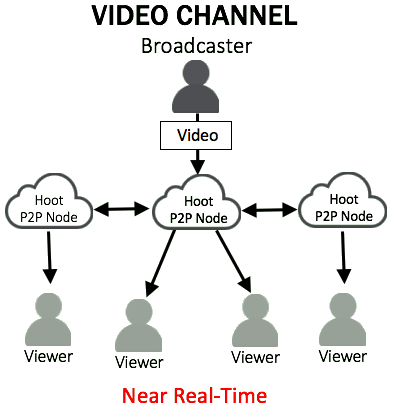
\includegraphics[scale=0.5]{static/hoot-video-architecture-channel-trans}

\subsection{Broadcast Side - mobile iOS client}
The protocol for realtime livestreaming video is called Real-Time Satoshi Streaming Protocol[\textbf{RTSSP}].
Video frames are captured at a resolution of 540x960 to 720x1280 based on network connectivity. Audio stream is captured using the built in iOS device microphone at a sampling rate of 44.1 KHz. Optionally, real time filters (Black and White, Glow, Fisheye, Sepia) can be applied to captured video frames in real-time. Video and audio are encoded using the native hardware H.264(H.265 in android) and AAC encoders, respectively. The video frames are encoded using a VBR algorithm with a maximum bitrate of 1 Mbps, this can be increased for usecases such as VR streaming. Audio stream is encoded in AAC format with a bitrate of 128 Kbps. The H.264 + AAC stream is encoded into an RTSSP stream and is transmitted to Hoot RTSSP server.

\subsection{Broadcast Side — Desktop Mac client}
Video frames are captured at native screen resolution, and audio stream is captured using the built in microphone at a sampling rate of 44.1 KHz. Hoot native cocoa Mac app written in Objective-C supports capturing FaceTime, Screenshare, and a combination of FaceTime and Screenshare. Video frames and audio stream are encoded using the native H.264 and AAC encoders, respectively. The video frames are encoded with a VBR algorithm. Audio stream is encoded in AAC format with a bitrate of 128 Kbps. The H.264 + AAC stream is encoded into an RTSSP stream and is transmitted to the open source RTSSP server.

\subsection{Viewer Side mobile iOS/Android client }
 Hoot open source Native mobile media player decodes RTSSP + H.264 and AAC data to make the live broadcast available to viewer in real-time. The HLS (HTTP Live Streaming) stream that is made available can be played using the iOS/Android Native media players, when the Hoot RTSSP player or app is not available.

\subsection{Viewer Side Mac/ Destkop PC client} 
The RTSSP stream is played using Adobe Flash technology supported by modern browsers. The HLS stream can be played using HTML5 player available in modern browsers.

\subsection{Server Side Peer-to-Peer decentralized Technology}
Similar to Bitcoin blockchain technology, any node can join or leave the Hoot network at anytime. Each node runs a realtime broadcasting server.
The GPUCoin network has several RTSSP servers that serve to bootstrap the Network. We use commodity servers with modern processors and with 1 Gbps duplex ethernet; specialized servers are not needed. The hoot server generates two variants of streams: a RTSSP stream and a HLS stream in order to make them accessible in browsers across Windows, Mac OS, Linux and Android platforms. A server with 1 Gbps duplex ethernet can support up to a total of 1000 viewers. A stream is replicated horizontally across multiple servers (without additional latency) to stream to virtually an unlimited number of simultaneous viewers. 

Streamed videos are instantly archived [\emph{H.264+AAC, mp4 container}] in the cloud for later viewing. The archived videos are indexed (scrubbable and quick to scan). We have access to datacenters in the following geographically distributed locations through RTSSP servers to provide the least latency to viewers globally: Amsterdam Netherlands, Frankfurt Germany, Hong Kong, London UK, Melbourne Australia, Queretaro Mexico, Milan Italy, Montreal Canada, Toronto Canada, Paris France, Singapore, Sydney Australia, Tokyo Japan, Dallas TX, Houston TX, San Jose CA, Seattle WA, Washington DC. 
% \sout{}
Streams are replicated and pulled to the closest node to the viewers location, i.e., a viewer in Tokyo Japan viewing a stream from Washington DC would be connected to a replicated stream on the Tokyo Japan hoot node in order to reduce latency.

